\documentclass[a4paper,12pt]{article}

\usepackage[a4paper,
            bindingoffset=0.2in,
            left=0.5in,
            right=0.5in,
            top=1in,
            bottom=1in,
            footskip=.25in]{geometry}

\usepackage{times}
\usepackage{graphicx}
\usepackage{xcolor}
\usepackage[acronym]{glossaries}
\usepackage{multirow}
\usepackage{authblk}

\makeglossaries

\newacronym{nlp}{NLP}{Natural Language Processing}
\newacronym{gpt}{GPT}{Generative Pre-trained Transformer}
\newacronym{qa}{QA}{Question answering}
\newacronym{ml}{ML}{Machine learning}
\newacronym{ai}{AI}{Artificial intelligence}
\newacronym{llm}{LLM}{Large Language Model}
\newacronym{dbqa}{DBQA}{Document-based question answering}
\newacronym{rnn}{RNN}{Recurrent neural network}
\newacronym{lstm}{LSTM}{Long-short term memory}
\newacronym{odqa}{ODQA}{Open-domain question answering}
\newacronym{ir}{IR}{Information retrieval}
\newacronym{abc}{ABC}{Asset-based consulting}

\author[1,2]{Hachem Betrouni}
\affil[1]{National Polytechnic school of Algiers, Industrial Engineering Department, Data Science and AI, Algiers, hachem.betrouni@g.enp.edu.dz}
\affil[2]{BIGmama technology, France, hb@big-mama.io}

\title{Document-based question answering}

\begin{document}
\maketitle
\begin{abstract}
In this thesis, we present a comprehensive analysis of various open-source embedding models and large language models (LLMs) for document-based question answering (DBQA). The goal of DBQA is to extract relevant information from a given document and answer user queries in natural language. We evaluate the performance of different embedding models, including BERT, E5, and MiniLM, in combination with open source LLMs such as Vicuna, Falcon, and OpenLlama.
Our experimental setup involves a retriever-generator framework, where a retrieval system retrieves the most relevant contexts from a document using embedding models. The conditioned generative system then generates a response to the user query based on the retrieved contexts using LLMs. We benchmark the performance of these systems using the SQuAD dataset.
We find that the choice of embedding model significantly impacts the retrieval performance. Moreover, we observe that the choice of LLM also plays a crucial role in generating accurate and informative answers.unsrt
This comparative analysis provides insights into the strengths and weaknesses of various open-source embedding models and LLMs for DBQA tasks. The findings of this study can guide researchers and practitioners in selecting suitable models for their specific DBQA applications and contribute to the advancement of question-answering systems.
\end{abstract}
\clearpage
\begin{center}
    \thispagestyle{empty}
    \vspace*{\fill}
    To my parents,\\
    to my family, mentors, friends, enemies, and every person who shaped who I am, \\
    to every rock that broke my bones, to every sea waving on the shores, \\  
    to Algiers's seagulls waking me up morning, reminded of Allah's boons,\\
    to Collo's men who rescued me,\\
    to you all I dedicate not this thesis but the years that led to its maketh.\\
    \vspace*{\fill}
\end{center}
\clearpage


\onecolumn
\tableofcontents
\listoffigures
\listoftables

\newpage
\printglossary[type=\acronymtype, title=List of acronyms]

\newpage

\section{General introduction}
For this BIGmama confined the development of a document-based question answering model to us.

\begin{figure}[h]
    \begin{center}
      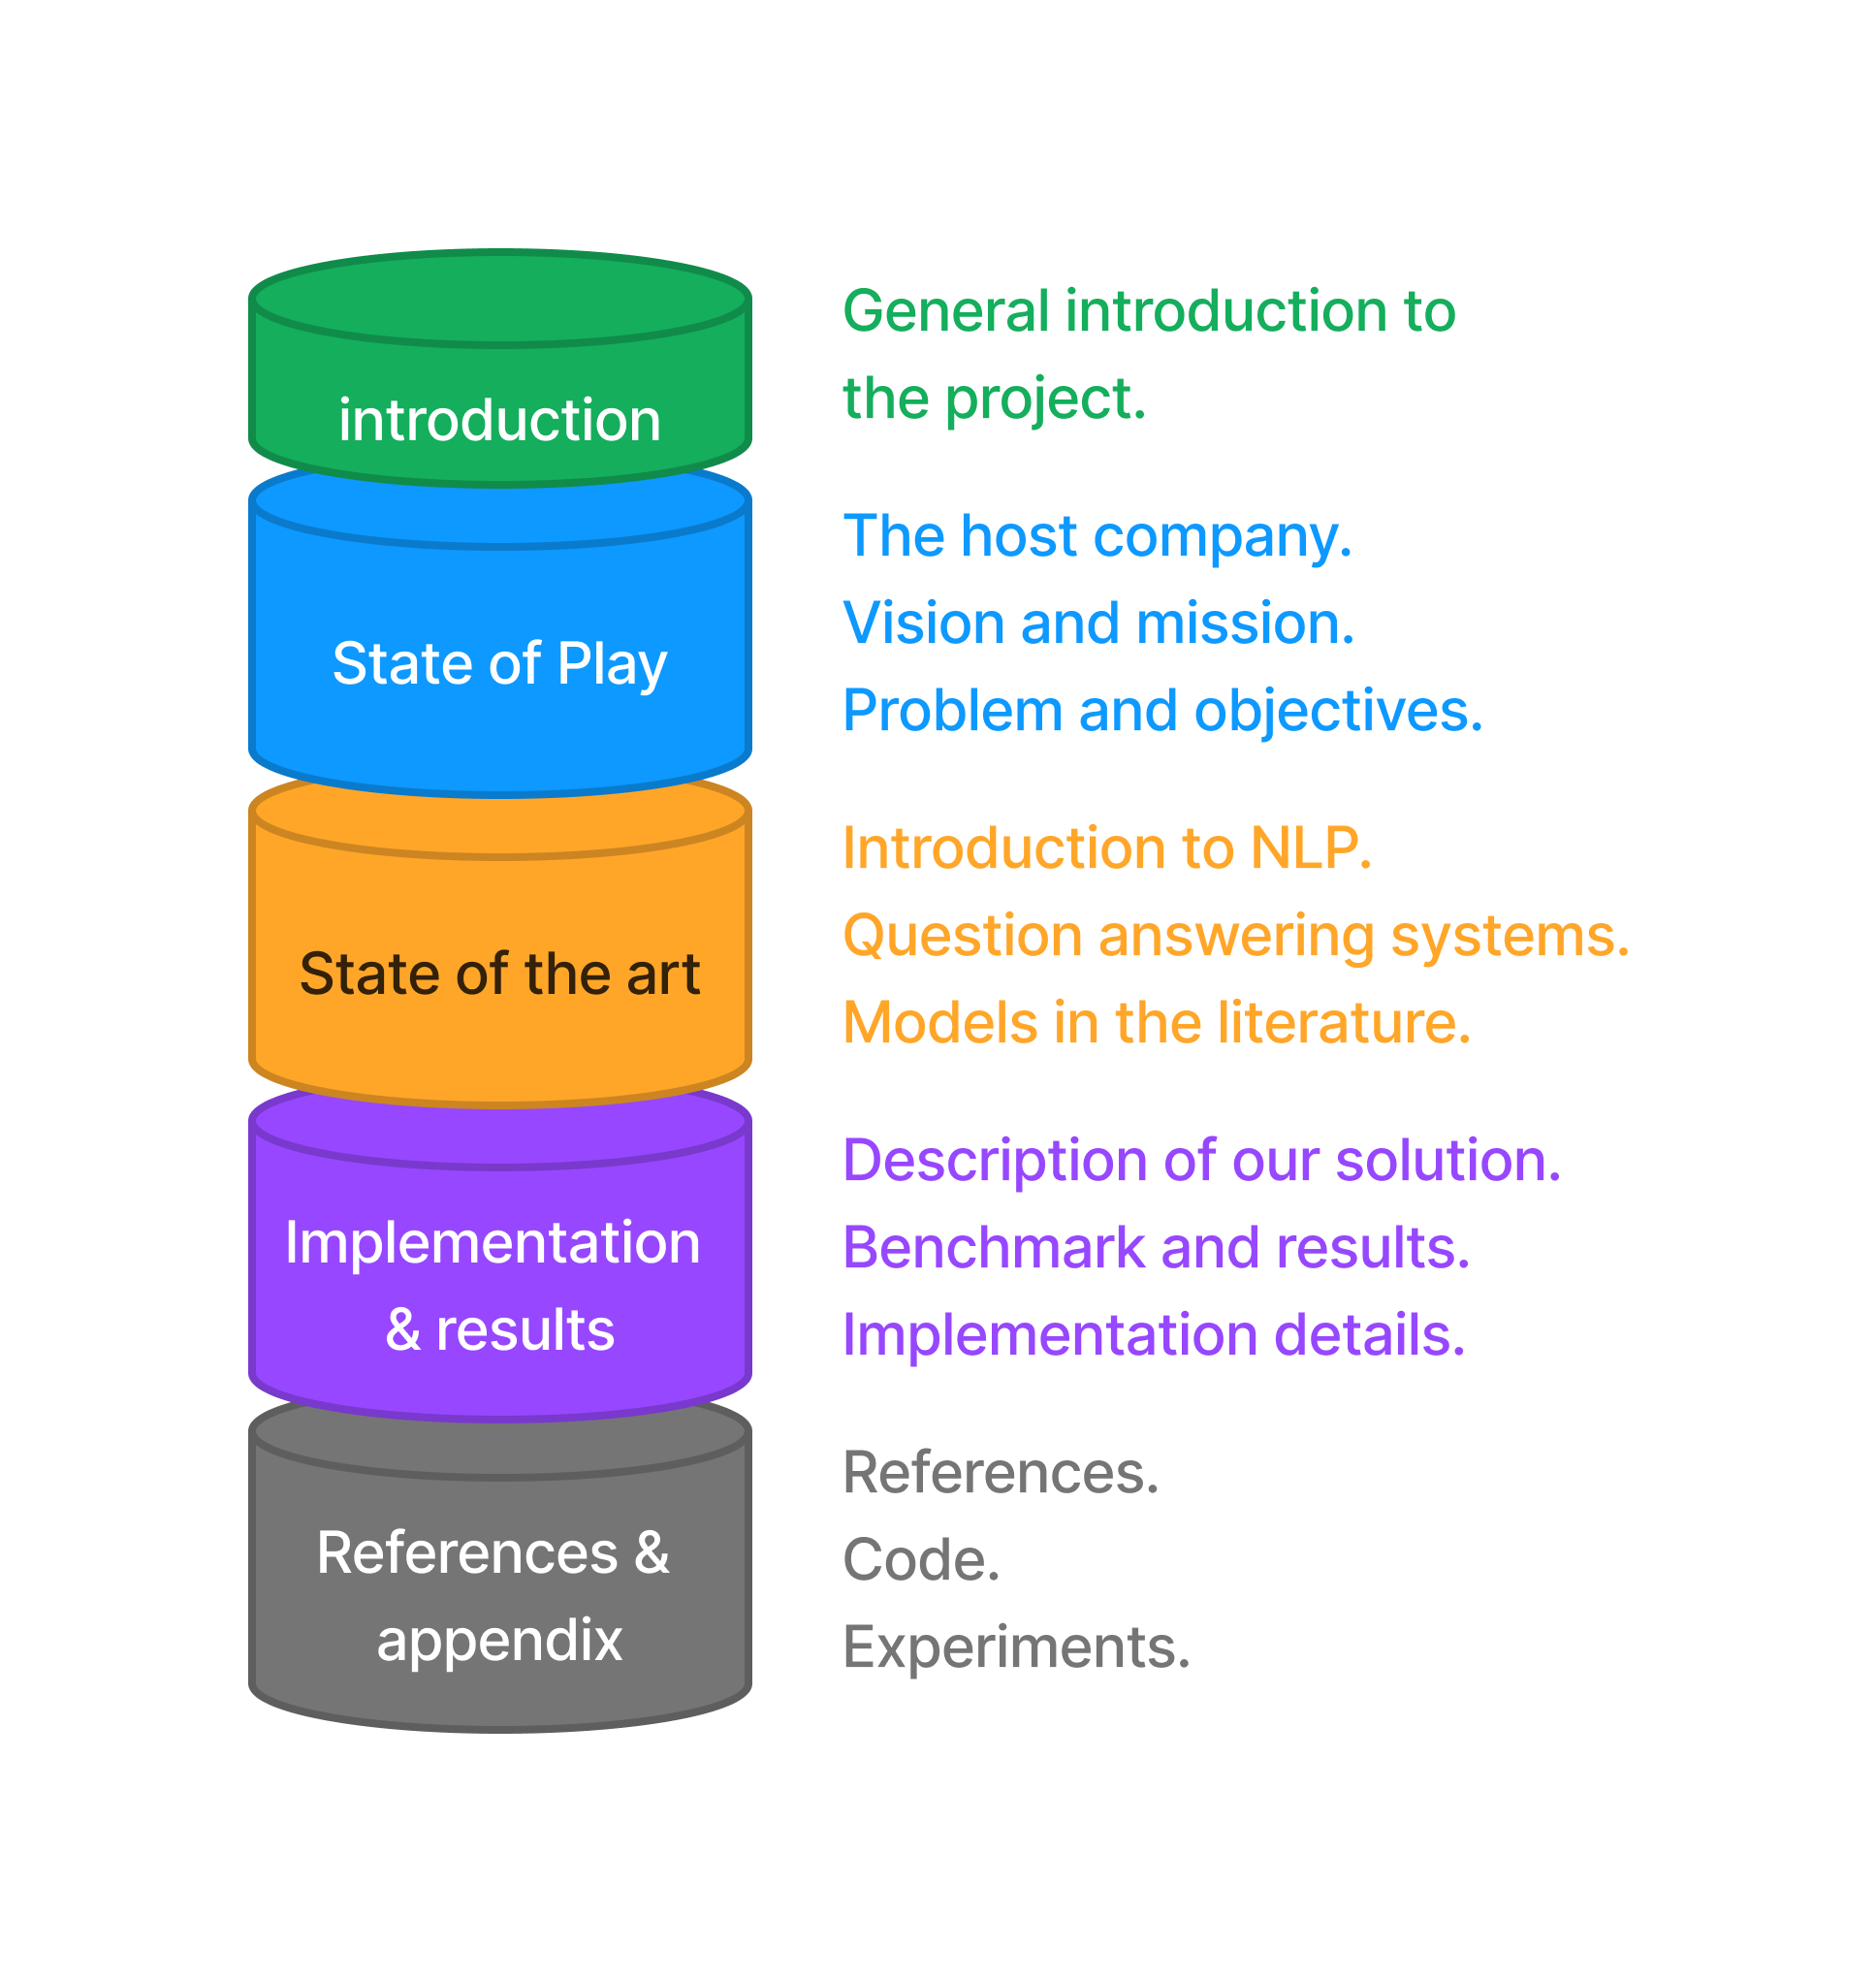
\includegraphics[width=0.4\textwidth]{figures/plan.png}
    \end{center}
  \caption{General structure of this document.}
    \label{fig:plan}
\end{figure}

\section{State of play}
\subsection{Introduction}
Creating value in the market is usually about solving a complex problem or answering a question. When it comes to the Data science and AI sector this used to be tackled with off-the-shelf solutions/applications/answers.
However the arrival of LLMs and other fundamental models upset the level of requirements. Creating value now requires expensive,  bespoke AI applications. The requirements are no longer to predict a number, but to explain the prediction, it's no longer to recommend a blog title but to generate its whole content.   

\subsection{Asset-based consulting}
This evolvement of the business landscape, driven by rapid technological advancements, changing market dynamics, and increasing competition created a fast-paced environment, where organizations seek innovative ways to optimize their operations, unlock hidden potentials, and achieve sustainable growth. 

Today we are well aware that answering these organizations needs for innovation has shifted from writing consulting reports (or any of the traditional approaches) to building tangible assets that concretize the added value. Today, clients are expecting specialised solutions to their problems, rather than the boilerplate solutions consultants traditionally provided.

This has given rise to a thriving industry known as asset-based consulting (ABC).

Asset-based consulting is a specialized field within consulting that focuses on identifying, leveraging, and maximizing the value of a company's assets, AI can be incorporated in the schema of consulting by leveraging the data/knowledge/expertise of the company, incorporating it with intelligent systems, automatize tasks and improve the productivity of its users in general. 

In the ABC context, assets can include tangible resources such as infrastructure, technology, and inventory, as well as intangible assets like intellectual property, brand equity, and human capital. By harnessing the full potential of these assets, asset-based consultants help organizations drive operational efficiency, enhance performance, and create a competitive advantage.

Unlike traditional consulting approaches that often emphasize external factors and strategies, asset-based consulting takes a more holistic and internal perspective. It recognizes that companies possess unique assets and capabilities that, when strategically managed, or in our case, combined with AI, can serve as the foundation for sustainable competitive advantage and resilience. Here consultants work closely with clients to understand their expertise, identify untapped questions and needs, and design tailored solutions.

Asset-based consulting is known for its multidisciplinary nature, drawing expertise from various fields including finance, operations, technology, marketing, and human resources. Consultants blend their industry knowledge, analytical skills, and business acumen to assess, diagnose, and unlock the hidden value with innovative assets. They often conduct thorough assessments, employ data-driven methodologies, and collaborate closely with expert teams to align the asset usefulness with the overall business objectives.

As industries become increasingly complex and competitive, the demand for asset-based consulting continues to rise. Organizations of all sizes and sectors recognize the need to unlock the value within their assets to stay ahead of the curve. From manufacturing firms seeking to optimize their supply chains to technology companies aiming to capitalize on their intellectual property, asset-based consulting provides a strategic framework and expertise to achieve these objectives.

\subsection{BIGmama technology}
BIGmama is a French registered startup with an Algerian extension, specialized in data science and AI. 
They have been developing bespoke predictive applications for more than 8 years (as of the year 2023).

The board of directors counts former CEOs of global groups (Danone, Safran) and the team is assembled from a dozen of high-level data scientists and software engineers.

\subsection{Mission}
BIGmama's mission is to democratize the access to bespoke AI applications, and to transform companies and individuals by introducing AI in their jobs however possible. 

From an original method based on the know-how developed while working with their partners for nearly a decade that we automate or increase with algorithms (Hybrid AI).

What is important at BIGmama today is to be able to industrialize this methodology by proposing a software that encapsulates and hybridizes this expertise with ML models. In this way, this tool will allows them to build state of the art predictive applications, relatively quickly and at an affordable cost.

They believe that a large part of the future of the AI sector will be played out in the ability to articulate human expertise with the countless possibilities offered by AI models.

The last version of the software they are developing (HYKO), should be released by this June.

\subsection{Vision}
Data science will soon become a commodity, the arrival of large language models (which are considered foundational models in NLP) mark but a start of a new wave of foundational models. In the near future, we can expect the emergence of generalist models that are equivalent to ChatGPT but specialized in computer vision tasks, forecasting, pattern recognition, and other domains.

AI projects that take 6 months in the making, require extensive "hyper-parameter tuning", hundreds of experiments, task specific architectural modeling, and that come at an expensive price will soon become obsolete and outdated.

The future is going to become in the hands of those who are capable of harnessing the power of these generalist models. Algeria and the whole African continent is far behind, and its no longer a question of closing this gap step by step, a "quantum jump" is required. BIGmama will lead this quantum jump, and will prove that excellence can beam from within the African continent. 

\subsection{Unique methodology}
One of the valuable heritages that BIGmama acquired during the 8 years of actively developing bespoke AI applications to its clients is a the unique methodology of work at BIGmama. it's centered around the idea is 

\subsubsection{AI starts with problematization.}
Data science does not start with data science but with a re-framing and problematization work. Our clients most often arrive with a subject (and not problems). A subject in it self is composed of many "hidden" problems (often hidden even to the client), a good consultant at BIGmama knows that this process of problematization (that of decomposing the subject into multiple problems) requires multiple iterations and attempts, and its success is deeply rooted to that of understanding the expertise of the client, their needs and to the skills of the consultant to translate these problems into something addressable by the current AI models.

\subsubsection{AI is a tool, not an end-goal}
At BIGmama, we firmly believe that AI should be seen as a powerful tool rather than an ultimate goal in itself. While AI technology continues to advance rapidly, its true value lies in its ability to address and solve specific problems or challenges faced by individuals, businesses, and society as a whole.
By recognizing AI as a tool, we emphasize its role in enabling and enhancing human capabilities rather than replacing them. And we emphasis that the current approaches in AI are not always the best to solve \textit{every} problem.

\subsubsection{Hybridization}
We believe that the future of AI lies in what is commonly referred to today as hybrid AI. This is a set of approaches and methodologies aimed at combining the potential of models with purely human knowledge. We believe that this hybridization allows us to put humans at the heart of technological development and to produce tools that are more efficient, easier to maintain, explain and that are far less expensive.

\subsection{Software as a service (SaaS)}
BIGmama is currently working on a software that intrinsically embeds its mission of democratizing AI and its unique methodology of how to do so. Hyko is an iterative software that help users formulate their problems properly using AI conversational systems powered by LLMs. It then automatically generate a working applications prototypes that combines and orchestrate multiple AI models predisposed in the user's model-base.

Hyko can be described as a three steps iterative process :

\paragraph{Diagnosis and problematization (Scoping)}

\paragraph{Automatic prototyping}
Hyko leverages the ever increasing availability of open-source AI models (Huggingface \cite{huggingface}, Github, etc.)
and the zero-shot reasoning capabilities \cite{zeroshot} of today's LLMs to solve the following tasks : 

\begin{enumerate}
    \item task planning : designing how the tasks should be addressed, setting up the inputs, outputs and the dependencies of each task in the pipeline.
    \item model selection : selecting the right model in each step of the pipeline.
\end{enumerate}

Similar to HuggingGPT \cite{hugginggpt}, by solving these tasks Hyko is capable of going from a description of the user's problems to a working AI prototype solution.


\paragraph{Enhancement of the prototype}


\begin{figure}[h]
\centering
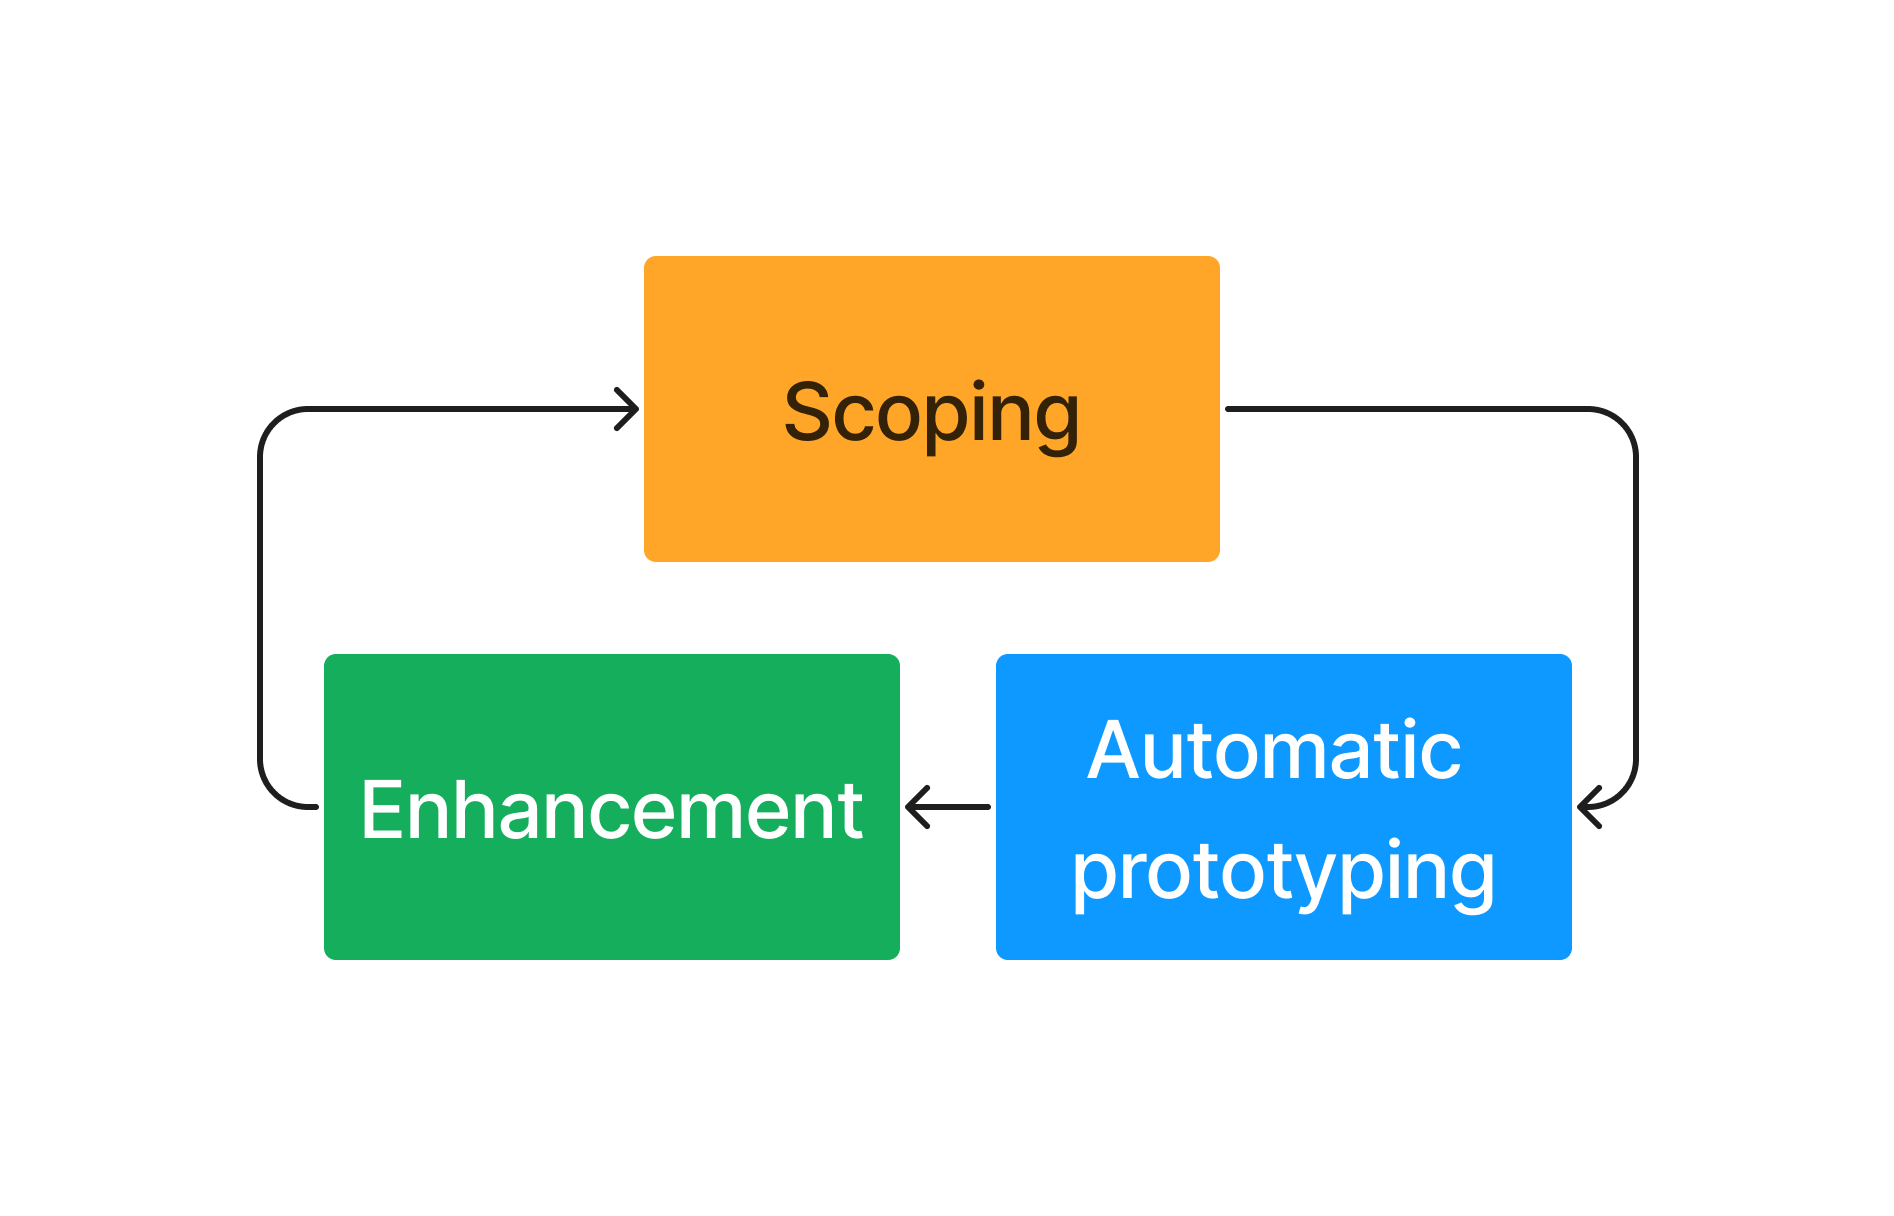
\includegraphics[width=.5\linewidth]{figures/3process.png}
\caption{Iterative process of developing an AI asset in Hyko.}
\label{fig:hykoprocess}
\end{figure}

\subsection{Knowledge representation}
A very important aspect of the first step (Scoping) is the ability to represent already existing knowledge (technical documents for example) and make it digestible by the LLMs behind the scoping phase.

\subsubsection{Document-based question answering}
Document-based question answering (DBQA) is a machine learning task that focuses on extracting accurate and relevant answers from a given document and responding in natural language to a specific query. 

It involves representing and manipulating content within textual documents, such as articles, technical documentation in order to provide precise answers to user queries.

DBQA systems typically involve a two stages process : 
\begin{enumerate}
    \item context retrieval : employing information retrieval (IR) techniques to extract relating contextual passages from the document.
    \item question answering (QA) : using natural language processing (NLP) approaches to answer a query using the retrieved context.  
\end{enumerate}  

\subsection{Conclusion}
In this paper we will dive deeper into the different frameworks, models and techniques used in DBQA systems (and similar QA tasks).

In this project we experimented with different DBQA systems, we prepared a small benchmark for few open-source LLMs used (in many combinations) with simple context retrieval systems.

\clearpage
\section{State of the art}

\subsection{Introduction}

\subsubsection{NLP Tasks}


\subsubsection{Embeddings}
A word embedding is a technique used in NLP to represent words as dense vectors in a high-dimensional space (an embedding). It aims to capture the semantic and syntactic relationships between words, enabling algorithms to process language more effectively.

Word embeddings can be created using two main approaches (or a combination of both): neural and statistical. 
Neural approaches, use neural networks to learn word representations by capturing semantic and syntactic relationships. Statistical approaches, rely on statistical features of words and their occurrences.

\paragraph{TF-IDF}
TF-IDF (Term Frequency-Inverse Document Frequency) is a commonly used weighting scheme in information retrieval and text mining tasks, designed to capture the importance of terms in a document collection. It combines two fundamental concepts: term frequency (TF) and inverse document frequency (IDF). TF refers to the number of times a term appears in a document, normalized by the total number of terms in that document. IDF, on the other hand, quantifies the rarity of a term across the entire document collection by taking the logarithm of the inverse of its document frequency. 

Document frequency refers to the number of documents in the collection that contain a given term. The TF-IDF weight for a term in a document is obtained by multiplying its TF value by its IDF value. This approach assigns higher weights to terms that appear frequently in a specific document but are relatively rare across the entire collection, effectively capturing their discriminative power. the TF-IDF weight of a term $t$ in a document $d$ can be computed as follows:

$${\displaystyle \mathrm {tf} (t,d)={\frac {f_{t,d}}{\sum _{t'\in d}{f_{t',d}}}}}$$
$$ \mathrm{idf}(t, D) =  \log \frac{N}{|\{d \in D: t \in d\}|}$$
$${\displaystyle \mathrm {tfidf} (t,d,D)=\mathrm {tf} (t,d)\cdot \mathrm {idf} (t,D)}$$


where $f_{t,d}$ is the raw count of a term in a document, i.e., the number of times that term $t$ occurs in document $d$,
$N$ the total number of documents in the corpus $N=|D|$ and  $|\{d \in D: t \in d\}|$ is the number of documents where term $t$ apears.

The resulting TF-IDF weights can be used for various purposes, such as document ranking, text classification, or keyword extraction, enabling the identification of important terms that characterize the content of documents in a collection.

\paragraph{Bert}
The BERT model \cite{bert} is pre-trained on large-scale corpora using unsupervised learning, followed by fine-tuning on specific downstream tasks. The resulting contextual word embeddings capture intricate semantic and syntactic relationships, enabling BERT to excel in various NLP tasks However BERT \cite{bert} uses a cross-encoder (i.e. two sentences are passed to the transformer network and the target value is predicted). This makes it unsuitable for various pair regression tasks due to too many possible combinations (finding most similar pair in a collection of $n$ sentences requires $\frac{n*(n-1)}{2}$ inferences). Sentence-BERT (SBERT) \cite{sbert}, is a modification of the BERT network using siamese and triplet networks, SBERT is able to
derive semantically meaningful sentence embeddings (semantically similar sentences are close in vector space).

\paragraph{E5}
According to Huggingface embedding models leaderboard \cite{embedding-leaderboard}, the E5 \cite{e5} is the current stat-of-the-art (average performance across 62 datasets and more than 7 tasks).

\paragraph{MiniLM}
MiniLM \cite{minilm} uses a simple and effective knowledge distillation method to compress large pre-trained Transformer based language models. The student model (MiniLM) is trained by deeply mimicking the teacher’s self-attention \cite{attention} modules,
which are the vital components of the Transformer networks.

The authors of \cite{minilm} propose using the self-attention distributions and value
relation of the teacher’s last Transformer layer to guide the
training of the student, which is effective and flexible for the student models. 

The embeddings that come from this model are of high quality, cheap to compute and can be used in a number of down stream tasks.

\subsubsection{Transformers}

Transformers are a type of deep learning model that have revolutionized natural language processing (NLP) tasks. They were introduced by \cite{attention} and have since become the state-of-the-art approach for various NLP applications.

\textbf{Attention Mechanism:}

Attention mechanisms are a key component of transformers. They allow the model to focus on different parts of the input sequence when processing each element. The attention mechanism assigns weights to each element in the input sequence based on its relevance to the current element being processed.

Given an input sequence $\mathbf{X} = \{x_1, x_2, \ldots, x_n\}$, the attention mechanism computes a weighted sum of all elements in $\mathbf{X}$, where the weights are determined by the relevance of each element to the current element. This can be mathematically represented as:

$$Attention(\mathbf{Q}, \mathbf{K}, \mathbf{V}) = softmax\left(\frac{\mathbf{QK}^T}{\sqrt{d_k}}\right) \mathbf{V}$$

where $\mathbf{Q}$, $\mathbf{K}$, and $\mathbf{V}$ are the query, key, and value matrices, respectively, and $d_k$ represents the dimension of the key.

\textbf{Multi-Head Attention:}

To capture different types of information, self-attention is performed multiple times in parallel, with different learned linear projections. The outputs of these attention heads are concatenated and linearly transformed:

$$
MultiHead(X) = Concat(head_1, head_2, ..., head_h)W_O
$$

where $head_i = SelfAttention(XW_{Qi}, XW_{Ki}, XW_{Vi})$, $W_{Qi}$, $W_{Ki}$, and $W_{Vi}$ are learnable weight matrices, and $W_O$ is the output weight matrix.

\textbf{Encoder Transformer:}

In a transformer model, the encoder is responsible for encoding the input sequence. It consists of a stack of identical layers, each comprising a multi-head self-attention mechanism and a feed-forward neural network. The encoder processes the input sequence in parallel and captures the dependencies between different elements.

Let $\mathbf{X} = \{x_1, x_2, \ldots, x_n\}$ be the input sequence. The encoder takes $\mathbf{X}$ and produces a sequence of encoded representations $\mathbf{Z} = \{z_1, z_2, \ldots, z_n\}$. The encoding process can be expressed as:

$$\mathbf{Z} = Encoder(\mathbf{X}) = EncoderLayer(\ldots(EncoderLayer(\mathbf{X})))$$

where $EncoderLayer$ represents a single layer in the encoder, and the ellipsis denotes the stacking of multiple layers.

\textbf{Encoder-Decoder Architecture:}

The encoder-decoder architecture extends the transformer model to tasks such as machine translation, where the input and output sequences have different lengths. The encoder processes the input sequence, while the decoder generates the output sequence.

Let $\mathbf{X} = \{x_1, x_2, \ldots, x_m\}$ and $\mathbf{Y} = \{y_1, y_2, \ldots, y_n\}$ be the input and output sequences, respectively. The encoder-decoder architecture can be summarized as:

$$\mathbf{Z} = Encoder(\mathbf{X})$$
$$\mathbf{Y'} = Decoder(\mathbf{Z}, \mathbf{Y}) = DecoderLayer(\ldots(DecoderLayer(\mathbf{Z}, \mathbf{Y})))$$

where $Decoder$ represents the decoder, $\mathbf{Z}$ is the encoded representation of $\mathbf{X}$ obtained from the encoder, and $\mathbf{Y'}$ is the predicted output sequence.

The decoder processes the output sequence $\mathbf{Y}$ and attends to the encoded representation $\mathbf{Z}$ to generate the output. The decoder also employs self-attention, allowing it to attend to previously generated elements in the output sequence.

\subsubsection{Similarity measures}
Similarity measures are used to quantify the degree of similarity or dissimilarity between two objects or vectors. They are widely used in various domains, including information retrieval, recommendation systems, and clustering. Different similarity measures capture different aspects of similarity based on the specific requirements of the task.

Here we mention a few examples of similarity measures commonly used in the litterateur. However the selection of a suitable similarity measure is contingent upon the characteristics of the data and the particular objectives of the task being performed.

\textbf{Cosine Similarity:}

Cosine similarity is a commonly used similarity measure that computes the cosine of the angle between two vectors. It is particularly useful when comparing the similarity between documents, text embeddings, or high-dimensional data. The cosine similarity between two vectors $\mathbf{A}$ and $\mathbf{B}$ can be calculated as:

$$cosine\_similarity(\mathbf{A}, \mathbf{B}) = \frac{\mathbf{A} \cdot \mathbf{B}}{\|\mathbf{A}\| \|\mathbf{B}\|}$$

where $\cdot$ denotes the dot product and $\|\cdot\|$ represents the Euclidean norm.

\textbf{Euclidean Distance:}

Euclidean distance is a commonly used dissimilarity measure that calculates the straight-line distance between two points in Euclidean space. It is widely used in clustering algorithms, such as k-means. The Euclidean distance between two vectors $\mathbf{A}$ and $\mathbf{B}$ of the same dimension can be computed as:

$$
euclidean\_distance(\mathbf{A}, \mathbf{B}) = \sqrt{\sum_{i=1}^{n} (A_i - B_i)^2}
$$

where $A_i$ and $B_i$ represent the $i$-th elements of vectors $\mathbf{A}$ and $\mathbf{B}$, respectively.

\textbf{Jaccard Similarity:}

Jaccard similarity \cite{jaccard} is a measure commonly used for comparing the similarity between sets. It is particularly useful in text mining and recommendation systems. The Jaccard similarity between two sets $A$ and $B$ is calculated as the size of their intersection divided by the size of their union:

$$
jaccard\_similarity(A, B) = \frac{|A \cap B|}{|A \cup B|}
$$

where $|A|$ and $|B|$ denote the cardinalities of sets $A$ and $B$, respectively.

\textbf{Hamming Distance:}

Hamming distance \cite{hamming} is a similarity measure used for comparing binary vectors of the same length. It calculates the number of positions at which the corresponding elements of two vectors are different. The Hamming distance between two binary vectors $\mathbf{A}$ and $\mathbf{B}$ can be computed as:

$$
hamming\_distance(\mathbf{A}, \mathbf{B}) = \sum_{i=1}^{n} (A_i \oplus B_i)
$$

where $A_i$ and $B_i$ represent the $i$-th elements of vectors $\mathbf{A}$ and $\mathbf{B}$, respectively, and $\oplus$ denotes the bitwise XOR operation.

\subsection{Many LLMs}
Plethora of large language models (LLMs) are being released week upon week. Some models are made open-source : OpenLlama \cite{openllama}, GPT-2 \cite{gpt2}, others are proprietary : GPT-3\cite{gpt3} and GPT-4 \cite{gpt4}, some are published for commercial use such as Falcon \cite{falcon}, others are only for research purposes : Llama \cite{llama} and Vicuna \cite{vicuna}.

Its hard to benchmark the performance of these models due to the wide range of applicable evaluation tasks and the difficulty of filtering out the genuine progress from grandiose claims as well as problems with current QA datasets and unrigorous evaluations \cite{unfairdataset}.

Huggingface recently published an LLM leaderboard \cite{open-llm-leaderboard}, where they evaluate publicly available LLMs on 4 key benchmarks : 

\begin{enumerate}
    \item AI2 Reasoning Challenge (25-shot) - a set of grade-school science questions \cite{AI2}.
    \item HellaSwag (10-shot) - a test of commonsense inference, which is easy for humans (~95\%) but challenging for SOTA models \cite{hellaswag}. 
    \item MMLU (5-shot) - a test to measure a text model’s multitask accuracy. The test covers 57 tasks including elementary mathematics, US history, computer science, law, and more \cite{MMLU}.
    \item TruthfulQA (0-shot) - a benchmark to measure whether a language model is truthful in generating answers to questions \cite{truthfulqa}.
\end{enumerate}

Most of the top performing models in this benchmark are either fine-tuned Falcon \cite{falcon} or fine-tuned LLama \cite{llama}.

\paragraph*{Falcon}
Large language models are typically trained using a combination of carefully selected high-quality data sources and filtered web data. 
The curation process aims to create models that perform well across a wide range of tasks. 
However, as the size of models increases and more training data is required, concerns arise regarding the scalability of the curation process and the availability of unique high-quality data.

The refined web dataset for Falcon llm \cite{falcondataset} demonstrates that properly filtered and deduplicated web data alone can yield powerful language models, 
even outperform state-of-the-art models trained on curated datasets like The Pile \cite{pile}. 
The authors of this dataset\cite{falcondataset} have released the Falcon \cite{falcon} language models with 1.3/7.5 billion parameters trained on this dataset, 
which serve as valuable resources for this project.

\paragraph*{LLaMa}
The authors of \cite{llama} present LLaMA, a collection of foundation language models with parameters ranging from 7 billion to 65 billion. 
They demonstrate that it is possible to train state-of-the-art models using publicly available datasets alone, without relying on proprietary or inaccessible data. 
In particular, LLaMA-13B surpasses the performance of GPT-3 (175B) \cite{gpt3} on most benchmarks, and LLaMA-65B is on par with other top models like Chinchilla-70B \cite{chinchilla} and PaLM-540B \cite{palm}. 
By making open-sourcing the LLaMA architecture and training code and by making the weights available for researchers, plenty of other models appeared as a result of fine-tuning the original LLaMA models on various tasks and datasets, 
these fine-tuned models include Alpaca \cite{alpaca} and Vicuna \cite{vicuna}. 

OpenLLaMa \cite{openllama} provides a totally open-source replication (weights and code, no research-only restriction) of the original LLaMA \cite{llama} models and which surprisingly in some cases outperforms the original models according to their benchmark \cite{openllama}     

\subsection{Question answering}
\subsubsection{Visual QA}
\subsubsection{Open-domain QA}
Open-domain Question Answering (ODQA) is a
task examining the ability of models to produce answers to natural language factoid questions drawn
from an open set of domains.

DrQA \cite{drqa} implemented Wikipedia as its knowledge source and this choice has became a default setting for many ODQA studies since then.

However it's relevant in some cases (such as ours) to limit the knowledge source to a signal (or multiple) pre-defined documents, there is a slight difference between the two tasks, to avoid confusion we call the latter "document-based question answering". 

Nevertheless approaches in ODQA are applicable for DBQA.

\subsection{Methods for document-based question answering}
\subsubsection{Open-book QA}
Open-book models in the field of Open-Domain Question Answering (ODQA) initially retrieve relevant documents then either extract or generate answers based on the information contained in the retrieved documents. We can distinguish mainly two approaches to tackle the ODQA problem :

\begin{enumerate}
    \item Retriever-reader : this model works toward finding the related context in the documentation than process the retrieved context to \textbf{extract} the start/end positions of an answer. The output of the model is the selected context and the identified span of the answer in the context. 
    \item Retriever-generator : unlike the reader model, the generator model generate free text conditioned with the retrieved context to answer the question.
\end{enumerate}

\paragraph{Retriever-reader}
Dense Passage Retrieval (DPR) \cite{dpr}, follows a pipeline approach, where documents are retrieved using dense embeddings. These retrieved documents are then passed to a conventional reader-re-ranker, which extracts specific spans of text as answers.

\paragraph{Retriever-generator}
Retrieval-Augmented Generation \cite{rag} is a seq2seq model that jointly learns to retrieve and generate answers. It utilizes dense retrieval and BART \cite{bart} for this purpose.


\begin{figure}[htbp]
  \centering
  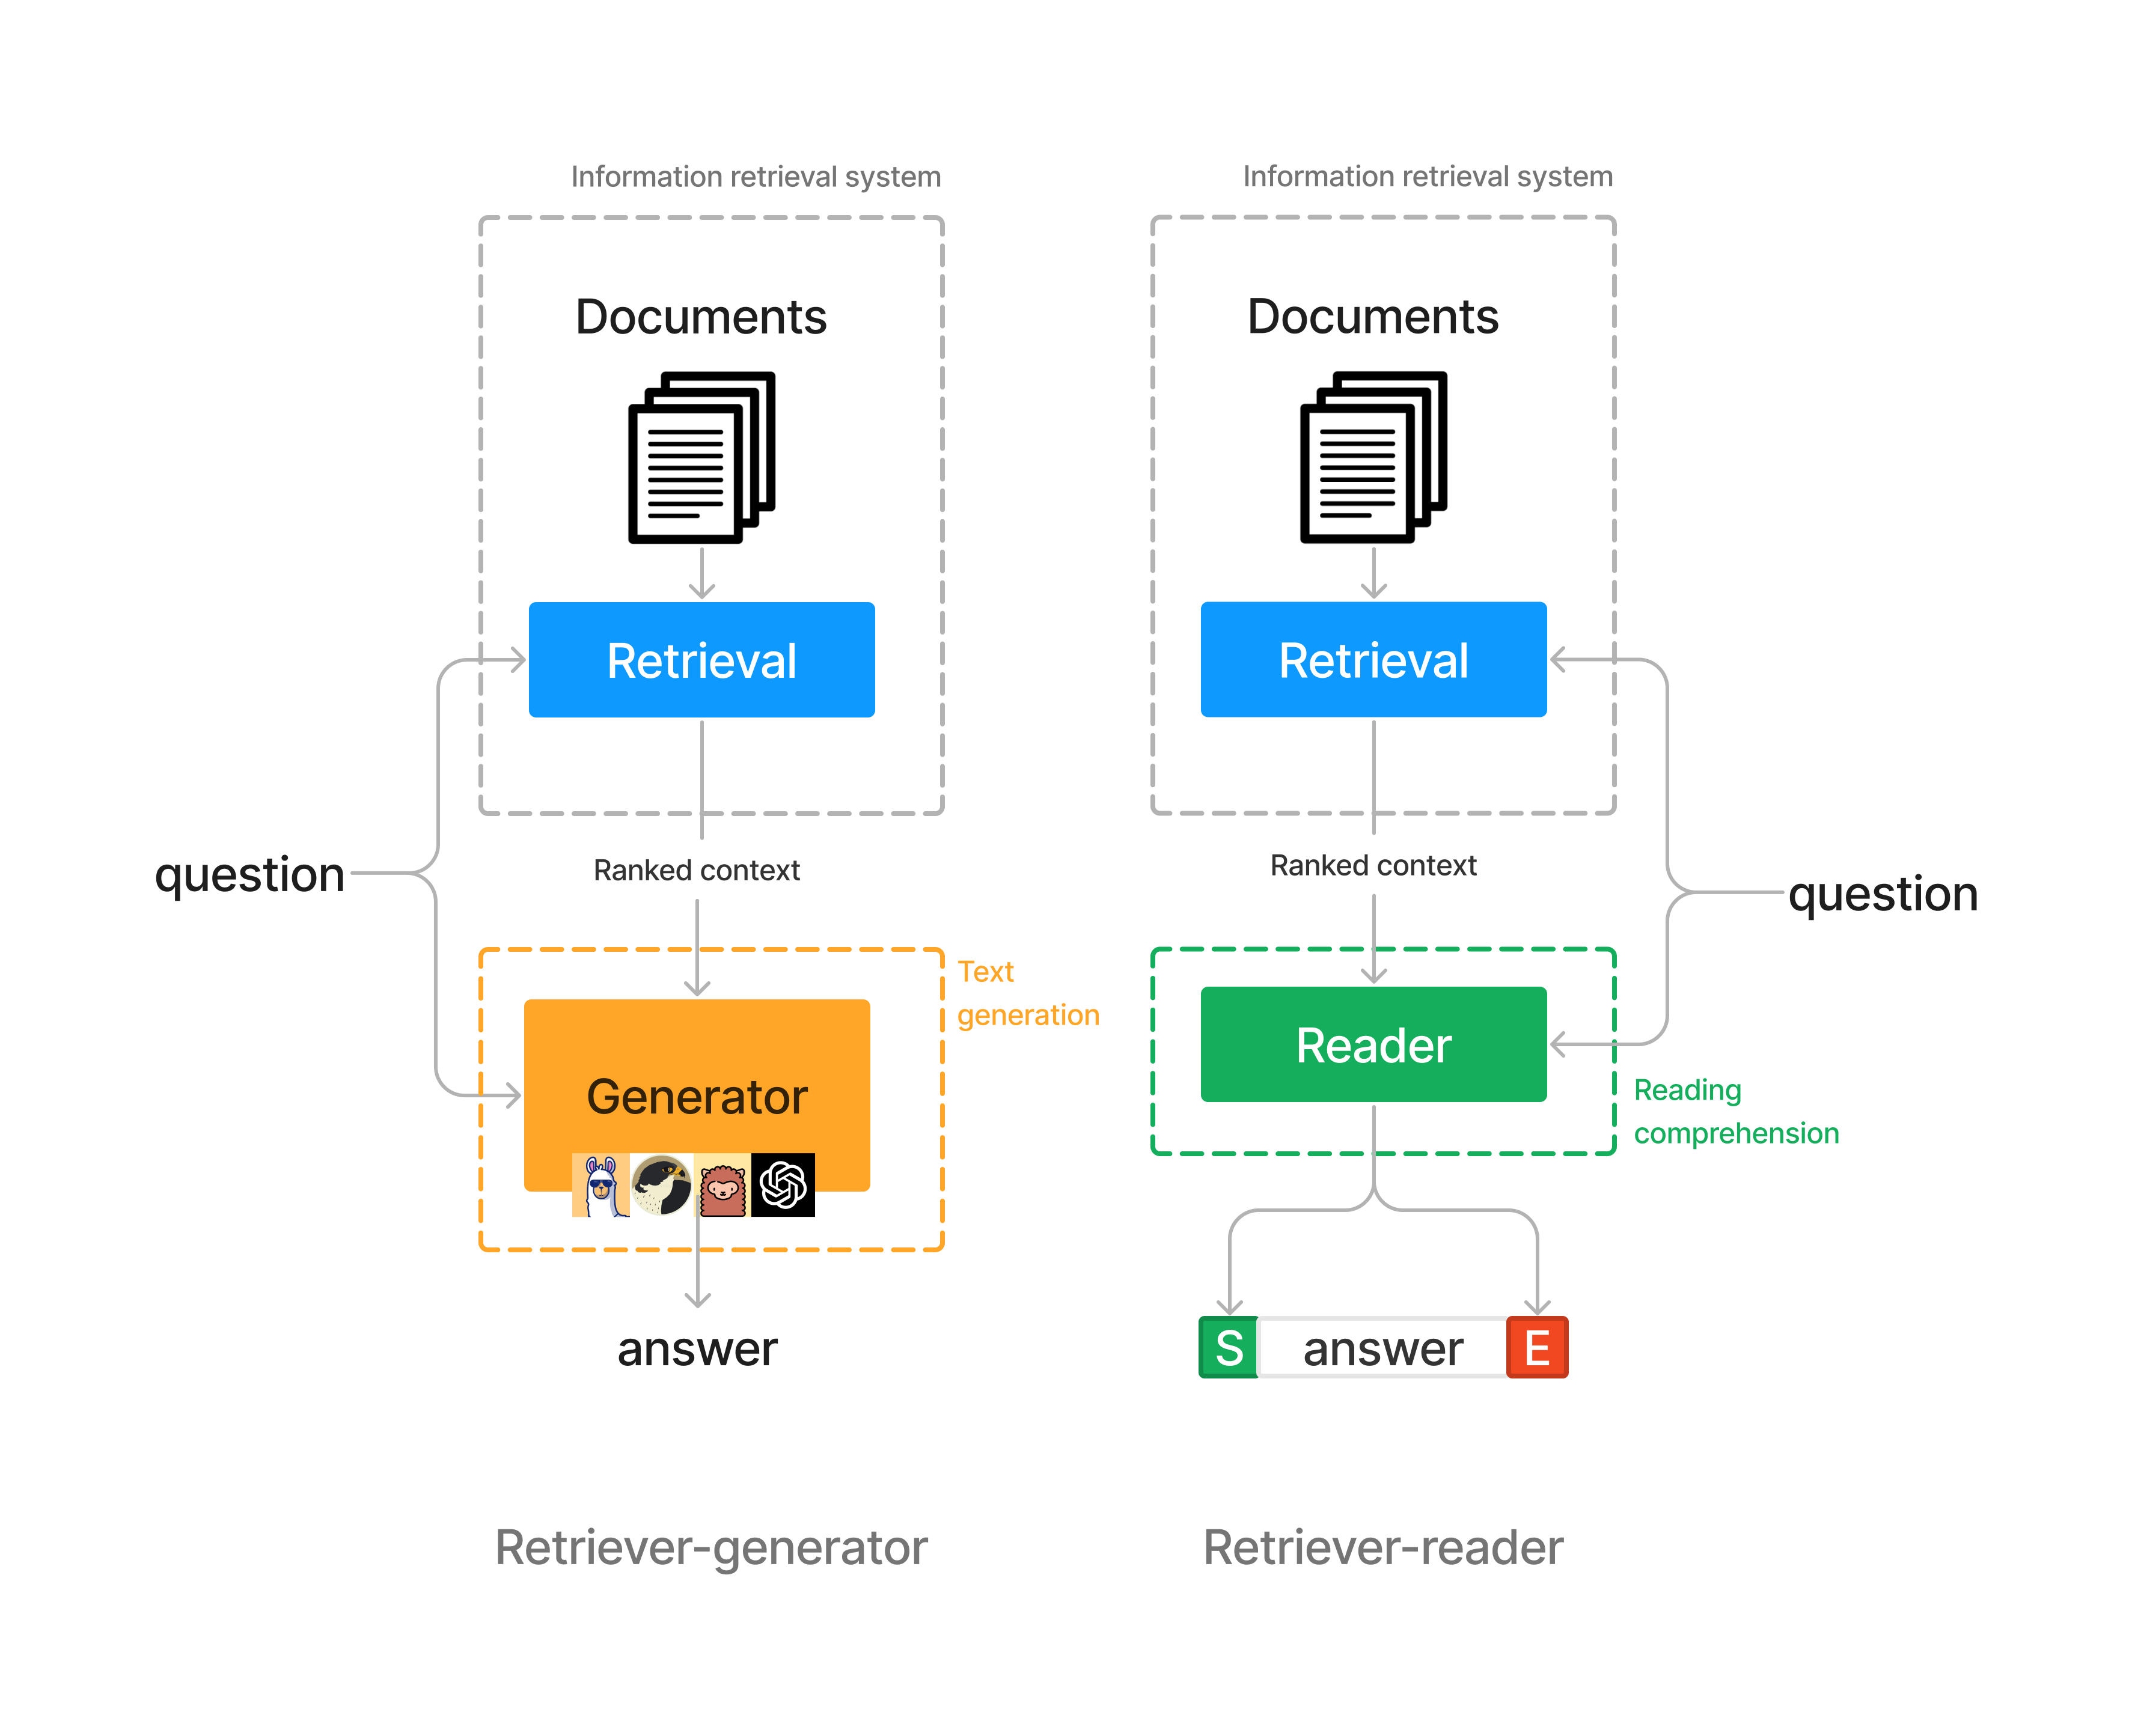
\includegraphics[width=0.8\linewidth]{figures/openbook.png}
  \caption{Overview of open-book question answering approaches.}
  \label{fig:openbook}
\end{figure}

\subsubsection{Closed-book QA}
Large language models undergo extensive unsupervised pre-training phase using large amount of textual data. With a substantial number of parameters, these models possess the ability to memorize factual information within their weight parameters. Consequently, one is able to employ this property for question-answering tasks without relying on explicit context (shown in figure \ref{fig:closedbook}). 

The pre-trained language models generate free-form text responses to questions, without explicitly employing reading comprehension techniques.
Closed-book models can encode the given documentation within the parameters of the model itself to answer queries, rather than using a retrieval model.

\begin{figure}
  \begin{center}
    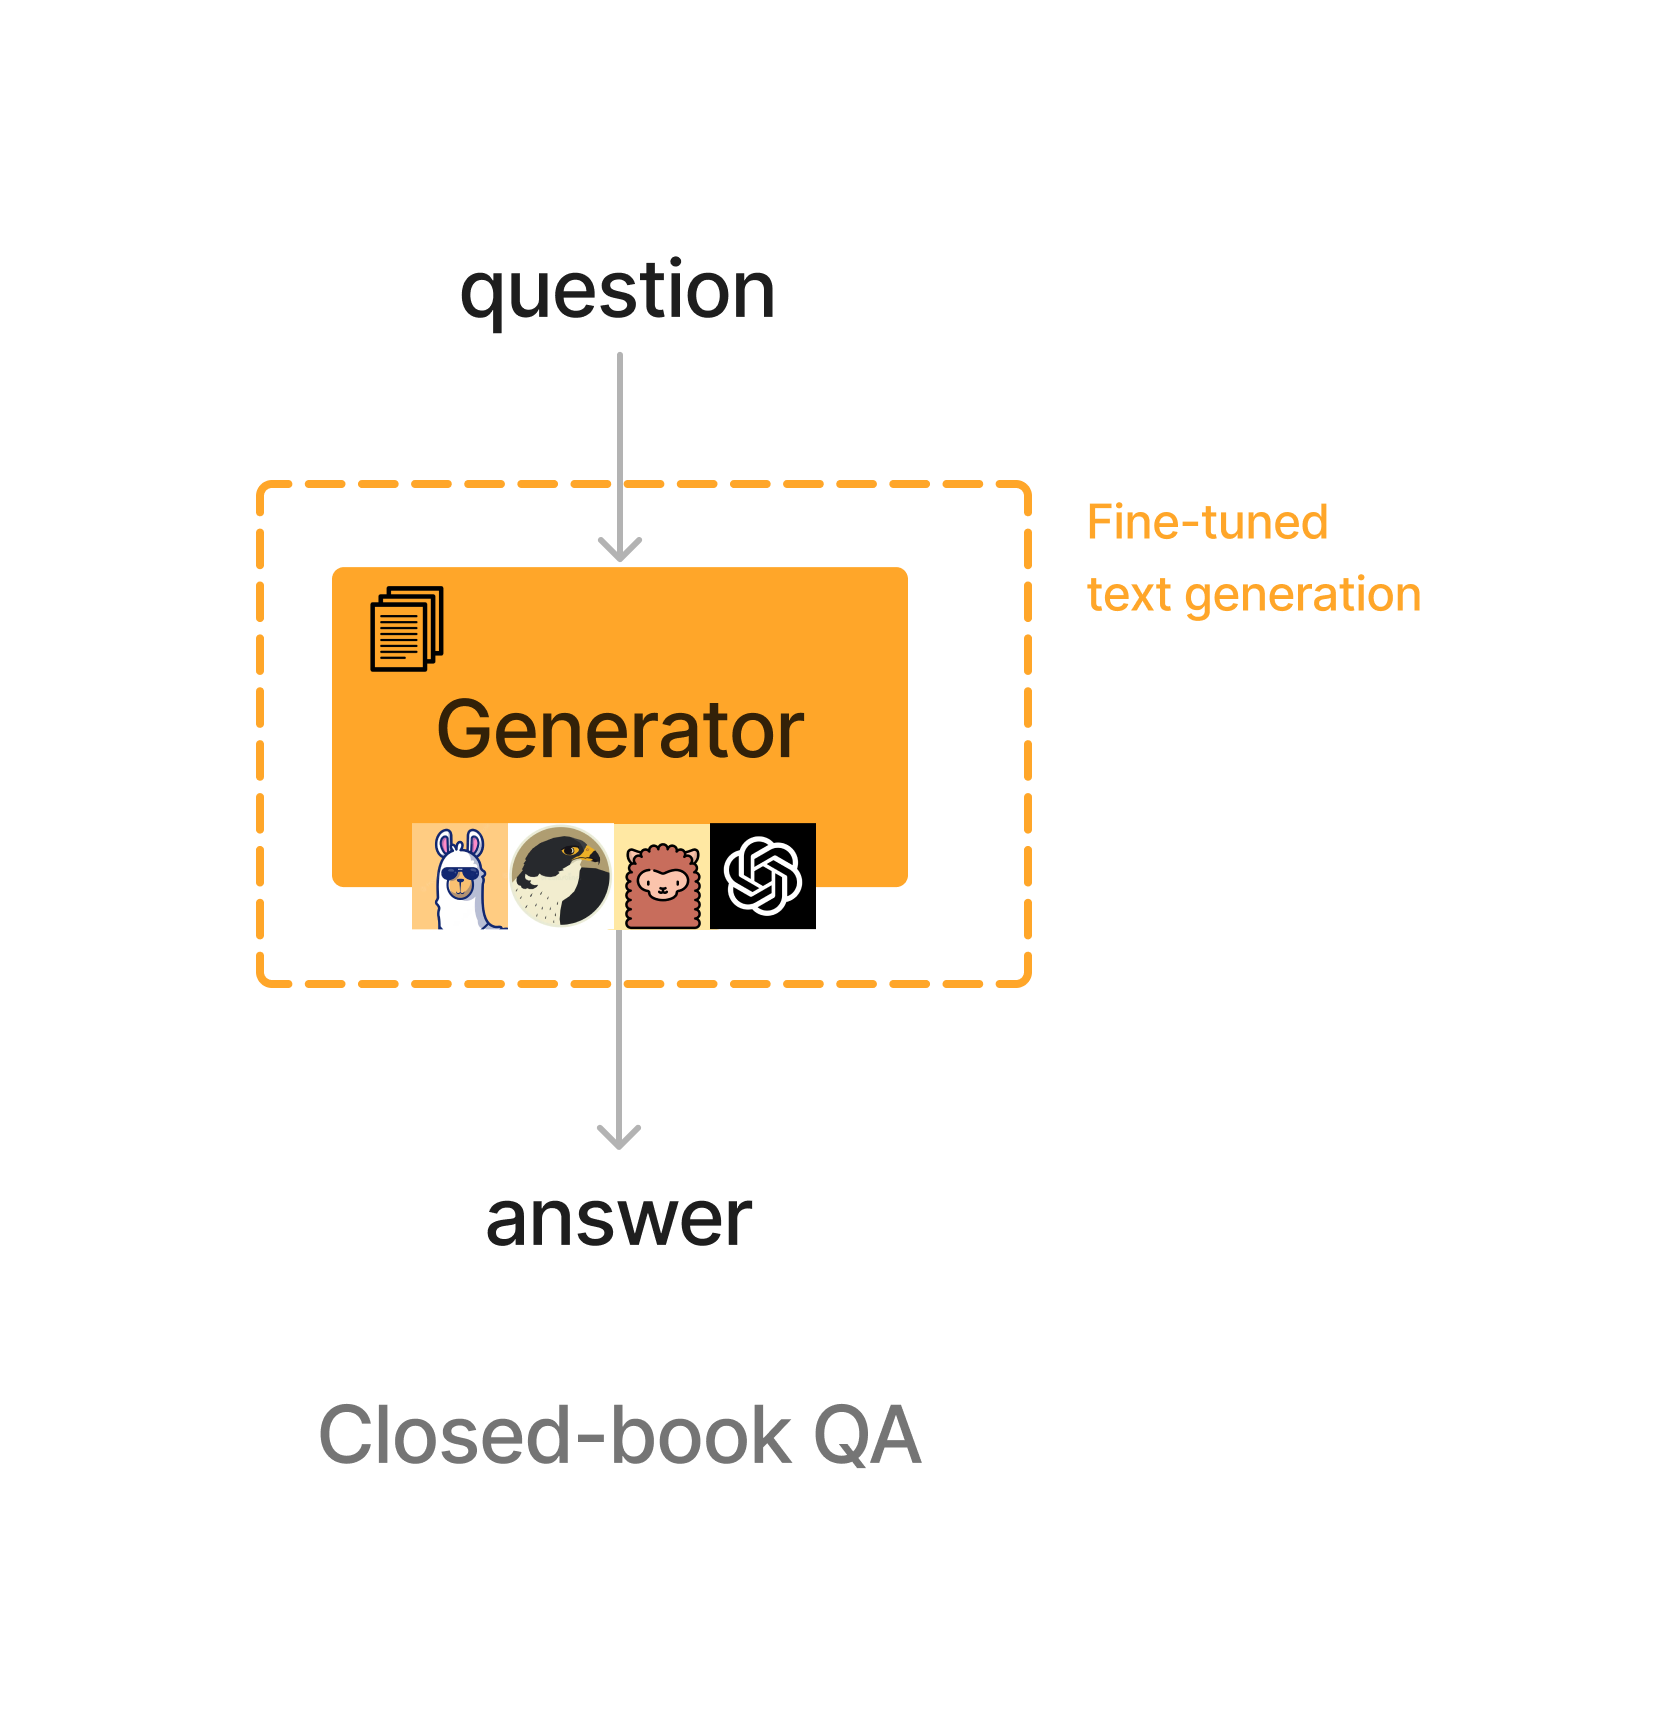
\includegraphics[width=0.4\textwidth]{figures/closedbook.png}
  \end{center}
\caption{Overview of closed-book fine-tuned QA.}
\label{fig:closedbook}
\end{figure}

Authors of \cite{T5Qa} fine-tune a pre-trained T5 \cite{T5} model to answer questions
(without access to any external context or knowledge) and were able (at the time) to compete with open-domain systems that
explicitly retrieve answers from an external knowledge source when answering questions.

GPT-3 \cite{gpt3} has been evaluated on the closed book question answering task using the TriviaQA dataset \cite{triviaqa} without any gradient updates or fine-tuning, the evaluation (figure \ref{fig:gpt3}) shows that GPT-3 match/exceed the performance of state of the art (at that time).

\begin{figure}
\centering
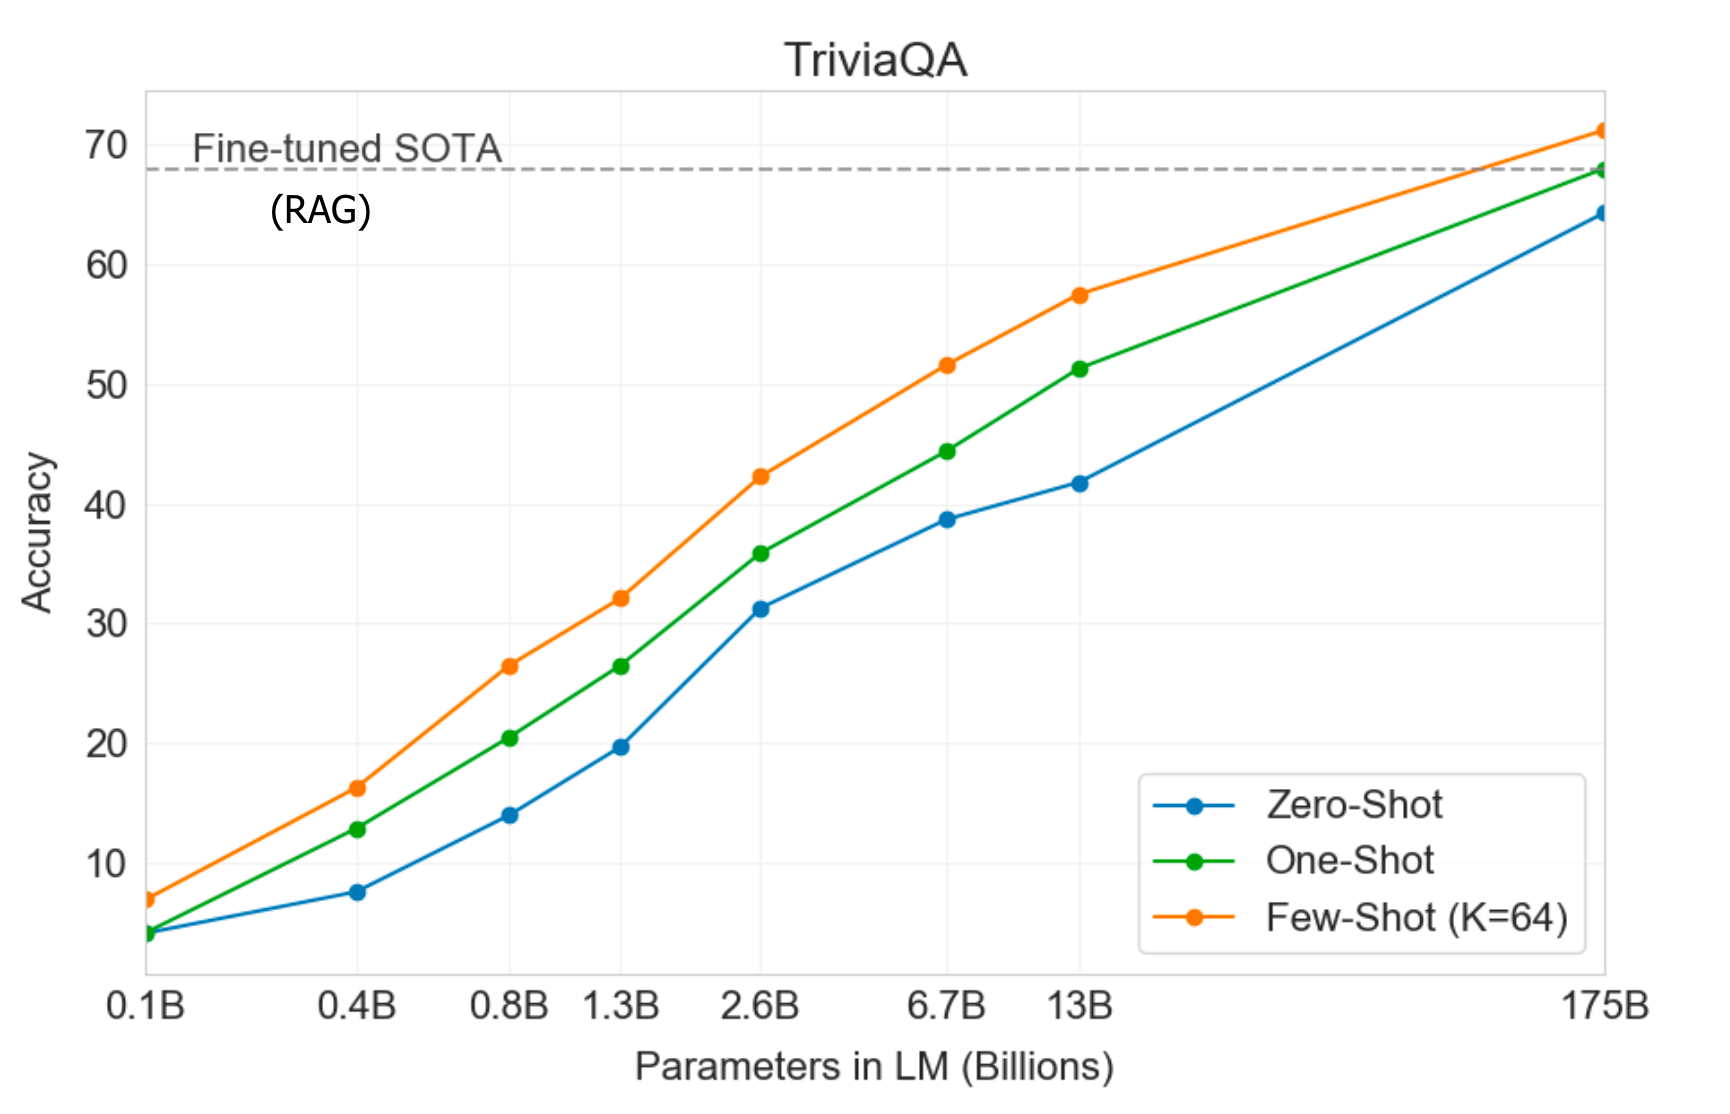
\includegraphics[width=0.8\linewidth]{figures/gpt3-triviaqa.png}
\caption{GPT3's performance on TriviaQA \cite{triviaqa}. \cite{gpt3}}
\label{fig:gpt3}
\end{figure}

\subsection{Retrieval models}
When it comes to implementing a retriever for a retriever-generator/retriever-reader models, there is mainly two systems : 
\begin{enumerate}
    \item using classic non-learning-based TF-IDF features (“classic IR”).
    \item or using dense embedding vectors of text produced by neural networks (“neural IR”).
\end{enumerate}

\paragraph{classic IR}
For example DrQA \cite{drqa} adopts an efficient non-learning-based search engine based on bigram hashing
and TF-IDF matching.

Another approach used by BERTserini \cite{BERTserini} consists of ranking retrieved text segments using BM25 \cite{BM25}, a classic TF-IDF-based retrieval scoring function.

In terms of the effect of text granularity on performance, \cite{BERTserini} found that paragraph retrieval > sentence retrieval > article retrieval.

Multi-passage BERT QA model \cite{multibert} uses elasticSearch with BM25 \cite{BM25}. They found that splitting articles into passages with the length of 100 words by sliding window brings $4\%$ improvements, and that splitting documents into passages without overlap causes some near-boundary evidence to lose useful contexts thus decreasing the performance.

\paragraph{neural IR}
Neural IR is a new category of methods for retrieval problems, it mainly uses dense representations of some neural network architectures (e.g. LSTM \cite{lstm}, BERT \cite{bert}, etc). 

After the arrival of many "general language models" (to do cite llms) many IR for QA systems follow this (or a slightly different) approach :
\begin{enumerate}
    \item Extract the dense representations of a question and a context passage by feeding them into a language model.
    \item Use the dot-product of these two representations as the retrieval score to rank and select most relevant passages.
\end{enumerate}

$$h_q=E_q(q)$$ 
$$h_z=E_z(z)$$
$$score=h_q^\mathsf{T} h_z$$

(however it is not necessary that neural IR out-performs classic IR \cite{lin})

\subsection{Reader Models}
The reader model objective is to learn solve reading comprehension tasks, extract an answer for a question from a retrieved context. 
Here we only discuss approaches for machine comprehension using neural networks since it yields best performing results.

\clearpage
\section{Implementation and results}
\subsection{Introduction}
LlamaIndex \cite{Liu_LlamaIndex_2022} bench-marked different indexing methods (different embeddings, LLMs and retrieval systems) following a similar approach to ours. However their focus was on OPENAI proprietary language models (GPT-3 and GPT-4) \cite{gpt3, gpt4}.
Our focus on the other hand was on using open-source embedding models and LLMs that can fully arun on-premise.

\begin{figure}[htbp]
\centering
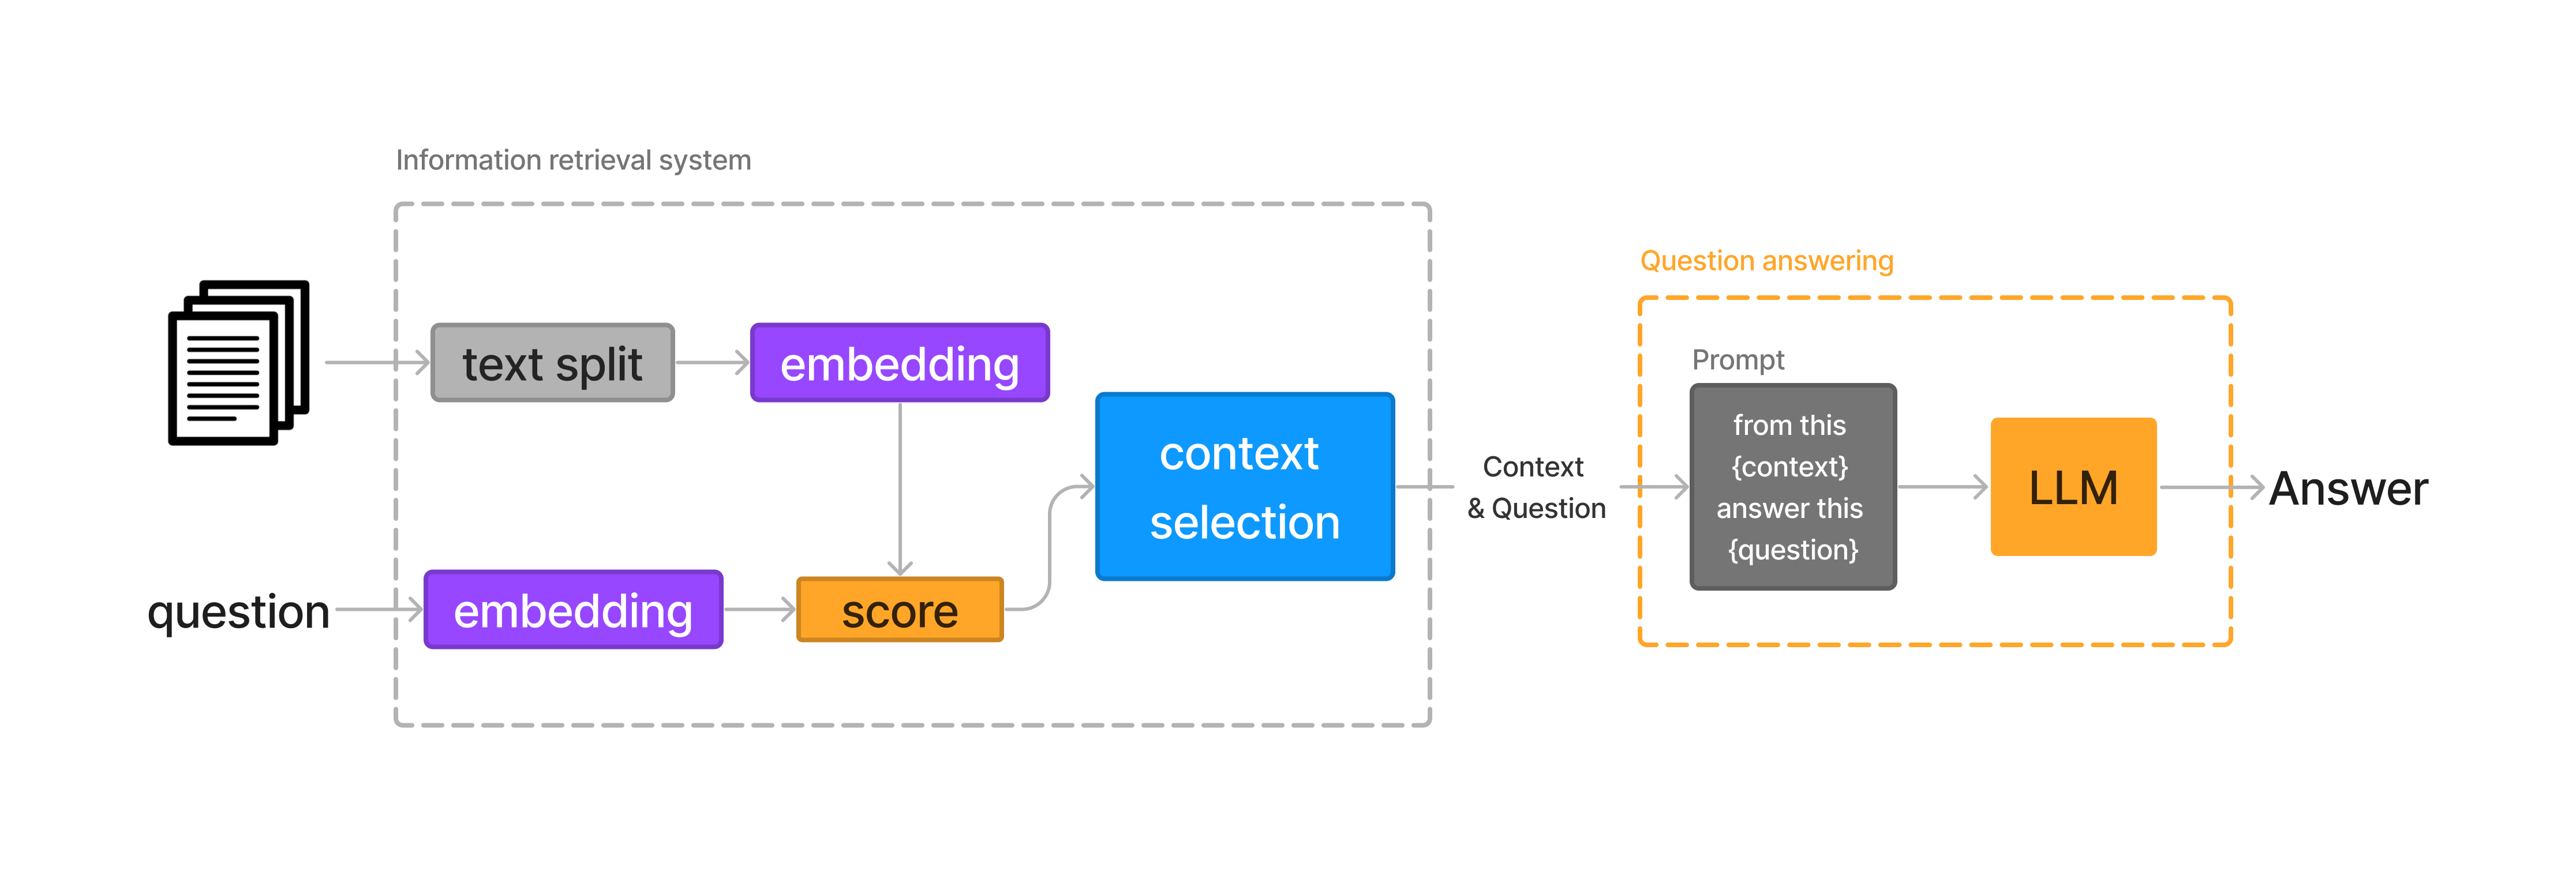
\includegraphics[width=.9\linewidth]{figures/full.png}
\caption{Highlevel overview of the whole system.}
\label{fig:overview}
\end{figure}

\subsection{Description}
The systems that we experimented with follows the retriever-generator framework, consists mainly of two parts : 

\paragraph{a retrieval system} that takes as input a document (text) and a query from the user, it splits the document into sentences using a heuristic algorithm developed for the processing the Parallel Corpus for Statistical Machine Translation \cite{europarl}. Each sentence from the document along the query of the user are going to be embedded by one of the chosen embedding models. We measure the one-to-one similarity (using cosine similarity) between the query embedding and each sentence embedding and we retrieve the top $K$ sentences to be used a context.

\paragraph{a conditioned generative system} it takes as input the retrieved contexts and the query to construct a prompt that condition the generation using one of the chosen open-source LLMs.
In table \ref{tab:benchmark} we show that we tested all the possible combination of the different embedding models and LMs at hand.

\subsection{Evaluation}
We bench-marked the different systems on the SQuAD dataset \cite{squad}. We sampled 20 with there context and answer (examples can be found in this annex \ref*{ann:experiments}), for each question and context 
we tested a different embedding and LLM, each response is them evaluated using GPT-3 \cite{gpt3} (a score of +1 is given if the answer is correct 0 otherwise), results are shown in table \ref{tab:benchmark}.

\begin{table}
    \centering
    \begin{tabular}{cccc}
        & & \color{orange}{\textbf{Language model}} & \\
        \cline{2-4}
        \color{violet}{\textbf{Embedder}} & \textbf{Vicuna} & \textbf{Falcon} & \textbf{OpenLlama} \\
        \hline
        Bert   & \textbf{0.4}  & 0.25 & 0.35 \\
        MiniLM & 0.35 & 0.25 & 0.3  \\
        E5     & 0.35 & 0.25 & 0.3  \\
    \end{tabular}
    \caption{Benchmark : score of each system when tested on 20 samples from SQuAD \cite{squad} dataset, and evaluated using GPT-3 \cite{gpt3}.}
    \label{tab:benchmark}
\end{table}

\subsection{Implementation details}

\section{Conclusion and perspectives}


\clearpage
% % Bibliography
\twocolumn
\bibliographystyle{plain}
\bibliography{references}
\clearpage

\onecolumn
\section{Annexes}
\subsection{Code}
\subsection{Experiments}\label{ann:experiments}
\end{document}